% CREATED BY DAVID FRISK, 2016
\chapter{Results}
\section{Experiment 1: Baseline Evaluation \& Blindfolding}
\begin{figure}
     \centering
     \begin{subfigure}[b]{0.4\textwidth}
         \centering
         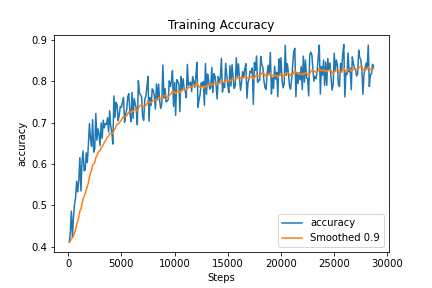
\includegraphics[width=\textwidth]{/home/yasmeen/Desktop/thesisproj/thesis/figure/results/baseline_and_blindfolding/training/accuracy.png}
         \caption{Training Accuracy}
         \label{fig:training_accuracy}
     \end{subfigure}
     \hfill
     \begin{subfigure}[b]{0.4\textwidth}
         \centering
         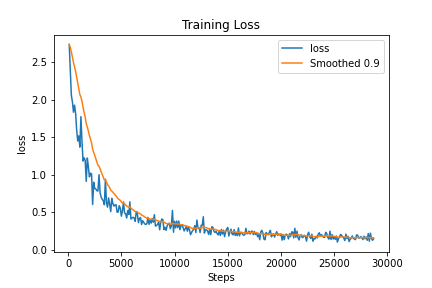
\includegraphics[width=\textwidth]{/home/yasmeen/Desktop/thesisproj/thesis/figure/results/baseline_and_blindfolding/training/loss.png}
         \caption{Training Loss}
         \label{fig:training_loss}
     \end{subfigure}
     \caption{Training Metrics}
     \label{fig:training_metrics}
\end{figure}

\begin{table}[h!]
\centering
\begin{tabular}{ |p{3cm}||p{3cm}|p{3cm}|  }
 \hline
 \multicolumn{1}{|c|}{Checkpoint} & \multicolumn{2}{|c|}{Evaluation} \\
 \hline
  & With Images & Blindfolded\\
 \hline
  & 
 ?   & ?    & ?\\
 \hline
\end{tabular}
\caption{Results of Baseline Evaluation}
\label{table:blindfolding results}
\end{table}
